\documentclass[a4paper,ngerman]{scrartcl}

\usepackage{amsmath}
\usepackage{amsfonts}
\usepackage{amssymb}
\usepackage[utf8]{inputenc}
\usepackage{graphicx}
\usepackage[ngerman]{babel}
\usepackage{hyperref}
\usepackage{float}
\usepackage{caption}
\usepackage{subcaption}
\usepackage{multirow}  %for tables
\usepackage{icomma} % Handle german comma as decimal point in numbers
\usepackage{units,siunitx} % Write units with correct spacing
\usepackage{upgreek} % provide non-italic greek letters
\usepackage{url}
%\usepackage{subfig}

% Formatting of table & figure captions
\captionsetup{font={sf,footnotesize},labelfont=bf,textfont=sl,skip=6pt}
\setlength{\abovecaptionskip}{6pt}
\setlength{\belowcaptionskip}{0pt}

\title{Magnetisierung\\Versuchsvorbereitung}
\date{\today}
\author{Michel Rausch, Michael Eliachevitch}

\begin{document}

\maketitle
\tableofcontents
\newpage

\section{Einleitung}

%Versuchsbeschreibung:
%Es wird die Magnetisierung von Selten-Erd-Metallen (Tb, Gd)im Temperaturbereich T = 77 - 300 K bestimmt. 
%Dazu wird ein supraleitendes Quanteninterferometer (Superconducting Quantum-Interference Device, SQUID) aus einem Hochtemperatursupraleiter verwendet, das sich in einem Flüssigkstickstoff-gekühlten Dewar befindet.

Mit einem supraleitendem Quanteninterferometer, einem sogenanntem
"`superconducting quantum interference device"' (\textbf{SQUID}), wird
die Magnetisierung der Seltenen-Erde-Metalle Terbium (\textbf{Tb}) und
Gadolinium (\textbf{SQUID}) über einen Temperaturbereich von $T=
\SI{77}{\kelvin}$ bis \SI{300}{\kelvin} bestimmt.
Das SQUID wird mit flüssigem Stickstoff gekühlt und befindet sich
daher in einem Dewar. In diesem Experiment werden die Grundlagen der
Supraleitfähigkeit und Magnetisierung vertieft und in einer Messung
angewandt.


\section{Theoretische Grundlagen}

\subsection{Supraleitung}

Supraleitung bezeichnet den Effekt, das einige Materialien, insbesondere Metalle, bei Unterschreitung einer Grenztemperatur $T_{\mathrm{C}}$ keinen Widerstand besitzen. 
Damit wird das Material diamagnetisch, Magnetfelder können nicht, oder nur gequantelt, in den Supraleiter dringen. 
Beim Überschreiten von $T_{\mathrm{C}}$ bricht die Supraleitfähigkeit zusammen. 

Die technischen Anwendungsmöglichkeiten sind weitreichend, jedoch meist in der Praxis durch $T_{\mathrm{C}}$ begrenzt, da die meisten Materialien mit flüssigem Helium gekühlt werden müssen, um supraleitend zu werden.
Andere Supraleiter, sogenannte Hochtemperatursupraleiter, werden bereits bei Temperaturen von flüssigem Stickstoff supraleitend. Jedoch bestehen sie meistens aus Keramiken statt aus Metallen und sind deswegen spröde und zum Beispiel für Drähte ungeeignet. 


\subsection{Cooper-Paare}

Für eine Supraleitfähigkeit müssen freie Elektronen vorhanden sein, daher tritt meistens in Metallen auf. % bei nieder-temperatur-supraleitern
Zusätzlich ist ein möglichst ideales Gitter notwendig.
Die Elektronen im Material besitzen Energien entsprechend einer Fermistatistik.
Elektronen nahe der Fermikante können, aufgrund einer schwachen anziehenden Wechselwirkung, sogenannte \textbf{Cooper-Paare} bilden, 
welche entgegengesetzte Spins und Impulse haben, sodass der Gesamtspin verschwindet und sie somit durch eine Bose-Einstein-Statistik beschrieben werden können.
Das Cooper-Paar lässt sich mit einer gemeinsamen Wellenfunktion beschreiben. 
Um diese zu stabilisieren, helfen Gitterschwingen, sogenannte (\textit{Phononen}). 
Bei konventionellen Supraleitern ist der gepaarte Zustand energetisch günstiger als der getrennte.
Es entsteht also eine Energielücke zwischen gepaarten und ungepaarten Elektronen. 

Die Stromdichte, bei der das Material widerstandsfrei leitet, ist begrenzt durch die sogenannte \textbf{kritische Stromdichte}, die temperaturabhängig ist.
Hochtemperatursupraleiter sind noch nicht vollständig verstanden und werden daher aktuell erforscht.



\subsection{Supraleiter im Magnetfeld}

Supraleiter lassen sich kategorisieren anhand ihrer Wechselwirkung mit Magnetfeldern. 
Ein Magnetfeld induziert Abschirmströme, die dem Magnetfeld entgegenwirken.
Als \textbf{Supraleiter 1. Art} bezeichnet man solche, die das Magnetfeld vollständig verdrängen (Meissner-Effekt, Kap. \ref{ssec:meissner}).  
Sie verdrängen das Magnetfeld im Inneren für geringe Feldstärken, bei extrem starken Magnetfeldern wird die Supraleitung zerstört.
Die meisten Supraleiter sind jedoch \textbf{2. Art}.
Magnetfelder können aufgrund der Josephson-Effekte (Kap. \ref{ssec:josephson}) durch Kanäle das Material passieren.

Man unterscheidet hier auch zwischen \textbf{"`harten"'} und \textbf{"`schwachen"'} Supraleitern.
Erstere besitzen besonders stabile Abschirmströme, frieren damit den magnetischen Fluss fest ein.
Schwache Supraleiter reagieren auf Änderungen des äußeren Magnetfelds und lassen magnetischen Fluss gequantelt mit einem Fluss von
\begin{equation}
\Phi_\mathrm{0} = \frac{h}{2 e}
\end{equation}
eindringen. 
Der Term "`$2 e$"' deutet auch auf ein Elektronenpaar hin.



\begin{figure}[tb!]
\centering
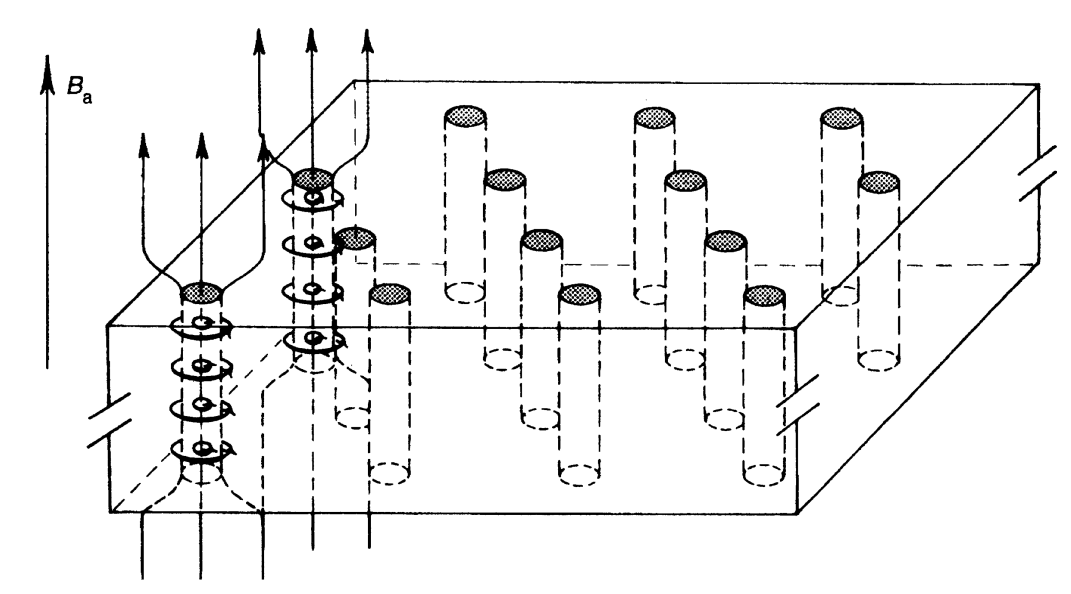
\includegraphics[width=0.7\textwidth]{abbildungen/typ2_supraleiter.png}
\caption[Versuchsplatz]{\textbf{Flussfadengitter in einem Typ II-Supraleiter [\ref{ref:mappe}].} Magnetfelder treten durch Kanäle in den Supraleiter ein. Die Flüsse sind quantisiert und verlaufen entlang der Magnetfeldrichtung.}
\label{fig:typII}
\end{figure}


\subsection{Meißner-Ochsenfeld-Effekt und Flussquantisierung in Supraleitern}
\label{ssec:meissner}
\paragraph{Der Meißner-Ochsenfeld-Effekt und Supraleiter 1. Art:}
Der Meißner-Ochsenfeld-Effekt bezeichnet die Eigenschaft von
Supraleitern 1. Art, externe Magnetfelder im supraleitenden Zustand,
unterhalb der kritischen Temperatur $T_C$,
aus ihrem Inneren vollständig zu verdrängen. Dieser Effekt tritt
sowohl dann auf, wenn das externe Magnetfeld bereits vor dem Erreichen
der Supraleitung vorhanden war und auch wenn das Magnetfeld erst nach
dem Erreichen der Supraleitung angelegt wird.

Dab der Supraleiter dabei dem externen Magnetfeld komplett
entgegenwirkt, hat er somit eine magnetische Suszeptibilität von $\chi
= -1$, womit er in dieser Phase ein perfekter Diamagnet ist. 

Überhalb einer kritischen Magnetstärke $B_C$ werden Supraleiter 1. Art
selbst bei Temperaturen $T < T_C$ wieder normalleitend.

Der Meißner-Ochsenfeld-Effekt ist neben dem verschwinden des
spezisischen Widerstandes eine grundlegende Eigenschaft von
Supraleitern und nicht klassisch erklärbar, sondern ein
makroskopischer quantenmechanischer Effekt. 

\paragraph{Flussquantisierung und Supraleiter 2. Art:}
Unter der kritischen Temperatur $T_C$ und bei externen magnetischen
Feldstärken $B < B_{C1}$ verhalten sich sogenannte Supraleiter 2. Art
genauso wie Supraleiter 1. Art und verdrängen gemäß dem
Meißner-Ochsenfeld-Effekt alle Magnetfelder in ihrem Inneren. 
Bei Magnetfeldern $B > B_{C2}$ mit $B_{C2} > B_{C1}$ geht auch bei
ihnen die Supraleitung verloren. 

Ihr besonderes Merkmal ist, dass sie in der Zwischenphase bei
Magnetfeldern der Stärke $B_{C1} < B < B_{C2}$ und Temperaturen $T <
T_C$ von Magnetfeldern durchdrungen werden können. 
Dabei handelt es sich um auch um einen makroskopischen
quantenmechanischen Effekt, da der Strom in der Leiterschleife bei der
Supraleitung durch Cooper-Paare erfolgt, die durch eine makroskopische
Wellenfunktion beschrieben werden. 


Da der Stromfluss Widerstandlos ist, gibt es keine Dämpfung und selbst
bei Abhandensein von äußeren Kräften fließt ein einmal angeregter
Strom in einer supraleitenden Spule immer weiter, was bedeutet, dass
er durch eine stationäre Wellengleichung beschrieben wird.
Aus der Quantenmechanik ist bekannt, dass stationäre Zustände in einem
System mit Randbedingungen diskrete Eigenwerte haben müssen.
Es folgt damit, dass der magnetische Fluss durch einen Supraleiter
quantisiert sein muss.

Das elementare Quant der Flusses lässt sich mithilfe der
Bohr-Sommerfeldschen Quantisierungsbedingung berechnen. 
Ein Teilchen mit der Stromdichte $\vec{j}$, der Ladung $q$ und der
Masse $m$ hat im Vektorpotential $\vec{A}$ den Impuls
\begin{equation}
  \begin{split}
      \vec{p} &= m \vec{v} + q \vec{A}\\
      &= \frac{m}{N q} \vec{j} + q \vec{A}~.
  \end{split}
\end{equation}

Integriert über die Leiterschlaufe mit der Quantisierungsbedingung
folgt damit

\begin{equation}
  \oint \vec{p} d\vec{s} = n \cdot h = \frac{m}{N q} \oint \vec{j}
  d\vec{s} + q \oint \vec{A} d\vec{s}~.
\end{equation}

Da Supraleiter nur an der Oberfläche leiten, verschwindet der Term 
$\oint \vec{j}d\vec{s}$ und mit dem Satz von Stokes erhalten wir

\begin{equation}
  n \cdot h = \oint \Delta \times \vec{A} d\vec{s} =
  q =: q n \Phi_0 ~.
\end{equation}

Damit erhalten wir die Quantisierungsbedingung

\begin{equation}
  \frac{n h}{q} = \oint\oint\vec{B}d\vec{F} = n \cdot \Phi_0~.
\end{equation}

Da Cooper-Paare die Ladung $q = 2e$ haben, folgt somit für Supraleiter
die Quantisierung 
\begin{equation}
  \label{eq:phi0}
  Phi_0 = \frac{h}{2 e} = \SI{2e-15}{\volt\second}~.
\end{equation}

Das passiert dabei so, dass der magnetische Fluss die supraleitende
Schlaufe in kleinen "`Tunneln"' dieser Größe durchlöchert.

\subsection{Josephson-Effekte}
\label{ssec:josephson}
Unter den Josephson-Effekten fasst man zwei weitere nur
quantenmechanisch erklärbare, makroskopische Eigenschaften von
Supraleitern zusammen. 
Sie treten auf, wenn man zwei Supraleiter durch eine dünne
isolierende (\emph{SIS}) oder normalleitende
Schicht (\emph{SNS}) voneinander trennt. 
In ersterem Fall würde man klassisch bei einer angelegten Spannung
$U_{\rm ext}$
keinen Stromfluss erwarten, da aber der Stromfluss mithilfe von
Cooper-Paaren in einem Supraleiter durch eine makroskopische
Wellenfunktion beschrieben wird, treten im supraleitenden Zustand
Tunneleffekte auf. 

Im folgenden betrachten wir der Einfachheit halber eine symmetrische
Anordung mit zwei identischen Supraleitern, die durch eine
Grenzschicht getrennt sind. 
In dem Fall lassen sich die beiden gekoppelten Schrödingergleichungen
des System mit der Energiedifferenz $\Delta E = e U$ zwischen den
Hälften berechnen. 
Wir wollen uns in dieser Vorbereitung nicht mit den Details der
Rechnung befassen, sondern betrachten direkt die Ergebnisse.

\paragraph{1. Der Josephson-Gleichstrom:}
Der erste Josephson-Effekt behandelt den Spannungslosen Fall mit
$U_{\rm ext} = 0$ 





\subsection{YBCO}

 


\section{Versuchsaufbau}

\subsection{SQUID}

Zur Messung der Magnetisierung wird ein "`superconducting quantum interference device"' (\textbf{SQUID}) der Firma Jülinger SQUID GmbH verwendet. 
Das verwendete SQUID basiert auf dem Hochtemperatursupraleiter Yttrium-Barium-Kupferoxid (\textbf{YBCO}).

\begin{figure}[tb!]
\centering
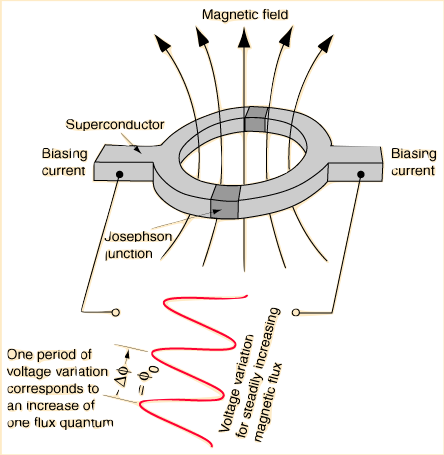
\includegraphics[width=0.7\textwidth]{abbildungen/squide.png}
\caption[Versuchsplatz]{\textbf{Aufbau eines dc-SQUIDs [\ref{ref:wuppertal}].} An einem supraleitendem Ring mit zwei Josephson-Kontakten wird ein Wechselstrom angelegt. 
Dieser induziert ein Magnetfeld durch den Ring. 
Ist das Magnetfeld zu stark, bricht die Supraleitfähigkeit zusammen.
Diese Änderung im Widerstand kann mit einem Resonanzkreis genau gemessen werden.}
\label{fig:squid_wuppertal}
\end{figure}

Verwendet wird ein rf-SQUID, der wie in Abbildung \ref{fig:jsq}. 
Dieser besitzt nur eine Schwachstelle in Form von gezielt eingebrachte Korngrenzen.
Die Dimensionierung des Bauteils erfolgte so, dass nur ein Flussquant passieren kann.
Bei nur wenigen Milliampère werden Stromdichten durch die Schwachstelle mit einer Größenordnung von \SI{e5}{A \per  \centi \square \meter}.
Bei einem rf-SQUID reicht eine einzelne induktiv gekoppelte Schwachstelle aus.

\begin{figure}[tb!]
\centering
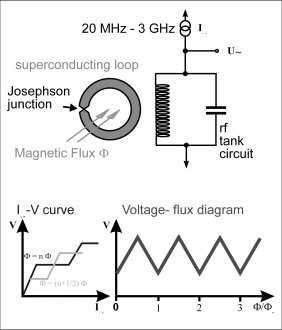
\includegraphics[width=0.7\textwidth]{abbildungen/squid_rf.png}
\caption[Versuchsplatz]{\textbf{Schema des rf-SQUIDs mit Kennlinien [\ref{ref:jsq}].} Das rf-SQUID wird mit einem Tank-Schwingkreis gekoppelt. Links unten ist die Abhängigkeit der gemessenen Spannung an dem Tankschwingkreis über den Pumpstrom aufgetragen. Rechts unten ist die Fluss zu Spannungs-Transferfunktion abgebildet.}
\label{fig:jsq}
\end{figure}



Angelegt wird eine hochfrequente Spannung von einigen \SI{100}{MHz}. 
Ein Tank-Schwingkreis ist induktiv mit der SQUID-Schleife gekoppelt und regt diese zur Schwingung an.
Es gilt für den magnetischen Fluss 

\begin{equation}
\Phi_{\mathrm{rf}} = M_\mathrm{G} \cdot Q \cdot I_{\mathrm{rf}} \cdot \sin(\omega_\mathrm{0} t) ~.
\end{equation}

$Q$ bezeichnet die Güte des Systems
\begin{equation}
Q = \frac{R_\mathrm{T}}{\omega_\mathrm{0} \cdot L_\mathrm{T}} ~.
\end{equation}
Die Gegeninduktivität ist mit den Induktivitäten $L_{\mathrm{SQ}}$ und $L_{\mathrm{T}}$ für SQUID-, bzw. Tankschwingkreis,
\begin{equation}
M_\mathrm{G} = k \cdot \sqrt{L_{\mathrm{SQ}} \cdot L_\mathrm{T}} ~.
\end{equation}
$k$ ist eine Koppelkonstante, $\omega_\mathrm{0}$ die Resonanzfrequenz und $R_\mathrm{T}$ der Widerstand des Tankkreises.

Gemessen wird die Amplitude der Erregerspannung $\Updelta U_{\mathrm{mess}}$.
Diese steigt mit $I_{\mathrm{rf}}$ linear an, solange der kritische Strom $I_\mathrm{C}$ von dem Suprastrom durch den SQUID $I_mathrm{S}$ nicht überschritten wird.
Wird der krtische Strom erreicht nd damit der kritische Fluss $\Phi_\mathrm{C}$, besitzt die Spannung einen kritischen Wert 
\begin{equation}
U_{\mathrm{C}} = \frac{\omega_\mathrm{0} \cdot L_\mathrm{T}}{M} ~.
\end{equation}

Der Supraleiter wird lokal normalleitend und der Schwingkreis verliert Energie an die Umgebung. 
Der Verlust beträgt etwa
\begin{equation}
\Delta E = I_\mathrm{C} \cdot \Phi_\mathrm{0} ~.
\end{equation}
Die Amplitude sinkt drastisch ab und der Vorgang beginnt erneut.


\subsection{Versuchsplatz}

Der Aufbau des Versuchsplatzes ist in Abbildung \ref{fig:Versuchsplatz} gezeigt.
Entsprechend dieser Anordnung soll der Versuch aufgebaut werden.



\begin{figure}[tb!]
\centering
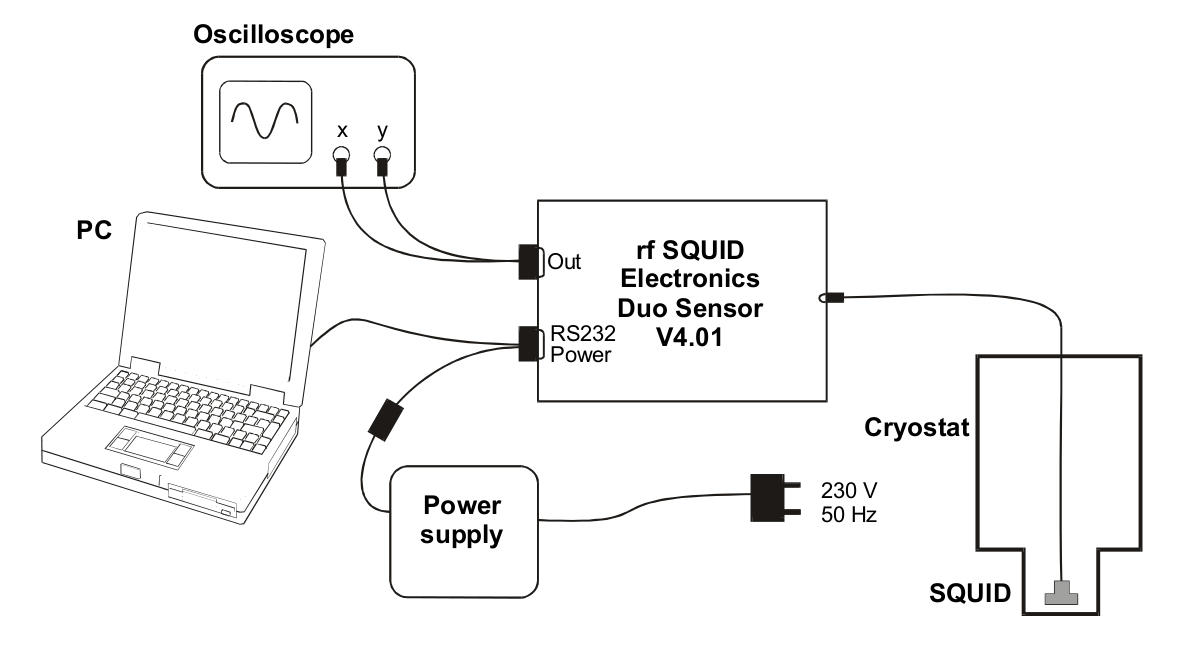
\includegraphics[width=0.7\textwidth]{abbildungen/aufbau_versuchsplatz.png}
\caption[Versuchsplatz]{\textbf{Aufbau des Versuchsplatz [\ref{ref:mappe}].} Das SQUID befindet sich in einem Dewar. 
Ein Sensor verwaltet die Spannungsversorgung und die Ausgänge zum Oszilloskop und PC.}
\label{fig:Versuchsplatz}
\end{figure}



\section{Versuchsdurchführung}

Der PC und die benötigte Software (DuoSensor.exe) wird gestartet.
Mit diesem Programm werden die Werte aufgenommen.
Die Arbeitspunktjustage wird, falls nicht schon vorhanden, durchgeführt.

Die Amplitude und Frequenz des Oszillators wird angepasst, dass die Schwingkreise gekoppelt sind.





\section{Quellen}
\begin{enumerate}
\item Vorbereitungsmappe.\label{ref:mappe}
\item \url{http://hydrogen.physik.uni-wuppertal.de/hyperphysics/hyperphysics/hbase/solids/squid.html} (18.1.2015).\label{ref:wuppertal}
\item \url{http://jsq.apps-1and1.net/category/information/what-is-a-squid/} (18.1.2015).
\label{ref:jsq}
\end{enumerate}



\end{document}
